\chapter{Vecteurs du plan}

\section{Translation et notion de vecteur}

\begin{definition}
	Soit $A$ et $B$ deux points distincts du plan. La translation qui transforme $A$ en $B$ est appelée \textbf{translation de vecteur $\vec{AB}$}.

	Lorsque $A$ et $B$ sont deux points distincts, le vecteur $\vec{AB}$ est caractérisé par :
	\begin{itemize}
		\item une \textbf{direction} : celle de la droite $(AB)$ ;
		\item un \textbf{sens} : de $A$ vers $B$ ;
		\item une \textbf{norme} (ou longueur) : la longueur $A B$, notée $\norm{\vec{AB}}$.
	\end{itemize}
	Le point $A$ est appelé \textbf{l'origine} du vecteur et le point $B$ son \textbf{extrémité}.

	\begin{center}
		\begin{tikzpicture}[>={Stealth[scale=1.2]}]
			\coordinate (A) at (0,0);
			\coordinate (B) at (4,1.5);
			\draw[dashed, color=gray] (-1,-0.375) -- (5,1.875) node[right] {$(AB)$};
			\draw[line width=1pt, ->] (A) -- (B) node[midway, above left] {$\vec{AB}$};
			\fill (A) circle (2pt) node[below] {$A$};
			\fill (B) circle (2pt) node[above] {$B$};
		\end{tikzpicture}
	\end{center}
\end{definition}

\begin{exemple}
	Sur le quadrillage ci-dessous (composé de carreaux de $1\text{ cm}$ de côté), plusieurs vecteurs ont été représentés :

	\begin{center}
		\begin{tikzpicture}[scale=0.8,>={Stealth[scale=1.3]}]
			% Quadrillage
			\draw[thin, color=gray!30] (0,0) grid (11,7);
			\coordinate (A) at (1,2);
			\coordinate (B) at (4,3);
			\draw[line width=1.2pt, ->, color=blue] (A) -- (B) node[midway, sloped, above,fill=white] {$\vec{AB}$};
			\fill (A) circle (2pt) node[below left] {$A$};
			\fill (B) circle (2pt) node[above right] {$B$};
			\coordinate (C) at (1,4);
			\coordinate (D) at (4,5);
			\draw[line width=1.2pt, ->, color=blue] (C) -- (D) node[midway, sloped, above,fill=white] {$\vec{CD}$};
			\fill (C) circle (2pt) node[below left] {$C$};
			\fill (D) circle (2pt) node[above right] {$D$};
			\coordinate (E) at (8,3);
			\coordinate (F) at (5,2);
			\draw[line width=1.2pt, ->, color=red] (E) -- (F) node[midway, sloped, above,fill=white] {$\vec{EF}$};
			\fill (E) circle (2pt) node[above right] {$E$};
			\fill (F) circle (2pt) node[left] {$F$};
			\coordinate (G) at (8,6);
			\coordinate (H) at (9,4);
			\draw[line width=1.2pt, ->, color=green!50!black] (G) -- (H) node[midway, sloped, above,fill=white] {$\vec{GH}$};
			\fill (G) circle (2pt) node[above left] {$G$};
			\fill (H) circle (2pt) node[below right] {$H$};
			\coordinate (I) at (4,1);
			\coordinate (J) at (10,3);
			\draw[line width=1.2pt, ->, color=orange!50!black] (I) -- (J) node[midway, sloped, below,fill=white] {$\vec{IJ}$};
			\fill (I) circle (2pt) node[below left] {$I$};
			\fill (J) circle (2pt) node[right] {$J$};
		\end{tikzpicture}
	\end{center}

	\textbf{Comparaisons des caractéristiques :}

	\begin{itemize}
		\item \textbf{Même direction, même sens et même norme :}
		      \begin{itemize}
			      \item Les vecteurs $\vec{AB}$ et $\vec{CD}$ ont la \textbf{même direction} : $(AB) \parallel (CD)$ ;
			      \item ils ont le \textbf{même sens} : vers la droite et vers le haut ;
			      \item ils ont la \textbf{même norme} : $\norm{\vec{AB}} = \norm{\vec{CD}} = \sqrt{3^2 + 1^2} = \sqrt{10}\text{ cm}$.
		      \end{itemize}

		\item \textbf{Même direction et même norme, mais sens contraire :}
		      \begin{itemize}
			      \item Le vecteur $\vec{EF}$ a la \textbf{même direction} que $\vec{AB}$ et $\vec{CD}$ : $(EF) \parallel (AB)$ ;
			      \item il a la \textbf{même norme} : $\norm{\vec{EF}} = \sqrt{10}\text{ cm}$ ;
			      \item en revanche, il est de \textbf{sens contraire} : vers la gauche et vers le bas.
		      \end{itemize}
	\end{itemize}
\end{exemple}

\begin{definition}
	Lorsque les points $A$ et $B$ sont confondus, la translation associée est la translation qui transforme $A$ en $A$.

	Le vecteur $\vec{AA}$ est appelé \textbf{vecteur nul} et est noté $\vec{0}$.
\end{definition}

\begin{remarque}
	Le vecteur nul n'a ni direction, ni sens, et sa norme est égale à $0$.
\end{remarque}

\section{Égalité de vecteurs et représentants}

\begin{definition}
	Soit $A$, $B$, $C$ et $D$ quatre points du plan. Dire que deux vecteurs $\vec{AB}$ et $\vec{CD}$ sont égaux signifie que le point $D$ est l'image du point $C$ par la translation de vecteur $\vec{AB}$.

	On note alors :
	\[
		\vec{AB} = \vec{CD}
	\]

	\begin{itemize}
		\item Il n'est pas toujours nécessaire de préciser l'origine et l'extrémité d'un vecteur : on désigne souvent un vecteur par une lettre minuscule surmontée d'une flèche, comme $\vec{u}$, $\vec{v}$ ou $\vec{w}$.
		\item Lorsque l'on écrit $\vec{u} = \vec{AB}$, on dit que le vecteur $\vec{AB}$ est un \textbf{représentant} du vecteur $\vec{u}$.
		\item Un même vecteur $\vec{u}$ possède une infinité de représentants dans le plan.
	\end{itemize}

	\begin{center}
		\begin{tikzpicture}[>={Stealth[scale=1.2]}]
			\coordinate (A) at (0,0);
			\coordinate (B) at (2.5,1);
			\draw[line width=1.2pt, ->, color=blue] (A) -- (B) node[midway, sloped, above] {$\vec{AB}$};
			\fill (A) circle (2pt) node[below left] {$A$};
			\fill (B) circle (2pt) node[above right] {$B$};
			\coordinate (C) at (4,0);
			\coordinate (D) at (6.5,1);
			\draw[line width=1.2pt, ->, color=blue] (C) -- (D) node[midway, sloped, above] {$\vec{CD}$};
			\fill (C) circle (2pt) node[below left] {$C$};
			\fill (D) circle (2pt) node[above right] {$D$};
			\coordinate (E) at (8,0);
			\coordinate (F) at (10.5,1);
			\draw[line width=1.2pt, ->, color=black] (E) -- (F) node[midway, sloped, above] {$\vec{u}$};
		\end{tikzpicture}
	\end{center}
\end{definition}

\begin{exemple}
	\nline
	\begin{wrapstuff}[r]
		\begin{tikzpicture}[scale=0.8,>={Stealth[scale=1.2]}]
			\draw[thin, color=gray!30] (0,0) grid (7,4);
			\coordinate (A) at (1,1);
			\coordinate (B) at (3,3);
			\coordinate (C) at (4,1);
			\coordinate (D) at (6,3);
			\draw[line width=1.2pt, ->, color=blue] (A) -- (B) node[midway, sloped, above] {$\vec{AB}$};
			\draw[line width=1.2pt, ->, color=blue] (C) -- (D) node[midway, sloped, above] {$\vec{CD}$};
			\draw[dashed, color=gray] (C) -- (D);
			\fill (A) circle (2pt) node[below left] {$A$};
			\fill (B) circle (2pt) node[above right] {$B$};
			\fill (C) circle (2pt) node[below left] {$C$};
			\fill (D) circle (2pt) node[above right] {$D$};
		\end{tikzpicture}
	\end{wrapstuff}
	On considère le quadrillage ci-contre.

	Pour passer du point $A$ au point $B$, on se déplace de $2$ carreaux vers la droite et de $2$ carreaux vers le haut.

	En partant du point $C$, si l'on applique ce même déplacement ($2$ carreaux vers la droite, $2$ carreaux vers le haut), on arrive exactement au point $D$.

	Le point $D$ est donc l'image du point $C$ par la translation de vecteur $\vec{AB}$.

	On en déduit que :
	\[
		\vec{AB} = \vec{CD}
	\]
\end{exemple}

\begin{exemple}
	\nline
	\begin{wrapstuff}[r]
		\begin{tikzpicture}[>={Stealth[scale=1.2]}]
			\coordinate (O) at (0,0);
			\coordinate (A) at (0:2);
			\coordinate (B) at (60:2);
			\coordinate (C) at (120:2);
			\coordinate (D) at (180:2);
			\coordinate (E) at (240:2);
			\coordinate (F) at (300:2);
			\draw[line width=1pt] (A) -- (B) -- (C) -- (D) -- (E) -- (F) -- cycle;
			\draw[dashed, color=gray] (A) -- (D);
			\draw[dashed, color=gray] (B) -- (E);
			\draw[dashed, color=gray] (C) -- (F);
			\node[below right,fill=white] at (O) {$O$};
			\fill (O) circle (2pt);
			\fill (A) circle (2pt) node[right] {$A$};
			\fill (B) circle (2pt) node[above right] {$B$};
			\fill (C) circle (2pt) node[above left] {$C$};
			\fill (D) circle (2pt) node[left] {$D$};
			\fill (E) circle (2pt) node[below left] {$E$};
			\fill (F) circle (2pt) node[below right] {$F$};
		\end{tikzpicture}
	\end{wrapstuff}

	On considère l'hexagone régulier $ABCDEF$ de centre $O$ ci-contre.

	Dans cette figure, bien que les vecteurs ne soient pas tous dessinés, on peut identifier de nombreuses égalités de vecteurs :

	\begin{itemize}
		\item \textbf{Vecteurs de même longueur que les côtés :}
		      \[
			      \begin{aligned}
				      \vec{AB} & = \vec{FO} = \vec{OC} = \vec{ED} \\
				      \vec{BC} & = \vec{AO} = \vec{OD} = \vec{FE} \\
				      \vec{CD} & = \vec{BO} = \vec{OE} = \vec{BA}
			      \end{aligned}
		      \]

		\item \textbf{Vecteurs portés par les petites diagonales :}
		      \[
			      \vec{FB} = \vec{EC} \quad \text{et} \quad \vec{AE} = \vec{BD}
		      \]
	\end{itemize}
\end{exemple}

\begin{propriete}[Vecteurs et parallélogramme]
	Soit $A$, $B$, $C$ et $D$ quatre points du plan.
	\begin{itemize}
		\item $\vec{AB} = \vec{CD}$ si, et seulement si, $ABDC$ est un parallélogramme (éventuellement aplati).
		\item $\vec{AB} = \vec{CD}$ si, et seulement si, $[AD]$ et $[BC]$ ont le même milieu.
		\item $\vec{AB} = \vec{CD}$ si, et seulement si, $\vec{AB}$ et $\vec{CD}$ ont la même direction, le même sens et la même norme.
	\end{itemize}

	\begin{center}
		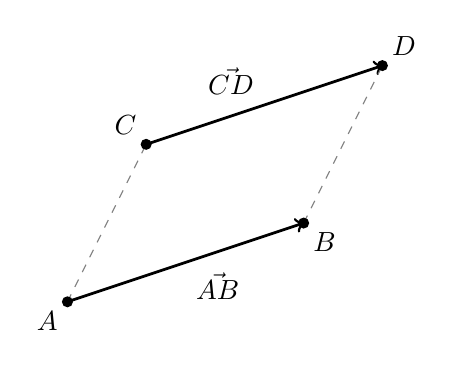
\begin{tikzpicture}[scale=1]
			\coordinate (A) at (0,0);
			\coordinate (B) at (3,1);
			\coordinate (C) at (1,2);
			\coordinate (D) at (4,3);
			\draw[line width=1pt, ->] (A) -- (B) node[midway, below right] {$\vec{AB}$};
			\draw[line width=1pt, ->] (C) -- (D) node[midway, above left] {$\vec{CD}$};
			\draw[dashed, color=gray] (A) -- (C);
			\draw[dashed, color=gray] (B) -- (D);
			\fill (A) circle (2pt) node[below left] {$A$};
			\fill (B) circle (2pt) node[below right] {$B$};
			\fill (C) circle (2pt) node[above left] {$C$};
			\fill (D) circle (2pt) node[above right] {$D$};
		\end{tikzpicture}
	\end{center}
\end{propriete}

\begin{propriete}[Vecteurs et milieu]
	Un point $I$ est le milieu d'un segment $[AB]$ si, et seulement si, $\vec{AI} = \vec{IB}$.

	\begin{center}
		\begin{tikzpicture}[>={Stealth[scale=1.2]}]
			\coordinate (A) at (0,0);
			\coordinate (I) at (2.5,0.8);
			\coordinate (B) at (5,1.6);
			\draw[line width=1.2pt, ->] (A) -- (I) node[midway, sloped, above] {$\vec{AI}$};
			\draw[line width=1.2pt, ->] (I) -- (B) node[midway, sloped, above] {$\vec{IB}$};
			\fill (A) circle (2pt) node[below right] {$A$};
			\fill (I) circle (2pt) node[below right] {$I$};
			\fill (B) circle (2pt) node[below right] {$B$};
		\end{tikzpicture}
	\end{center}
\end{propriete}

\begin{exemple}
	Soit $ABCD$ un parallélogramme de centre $I$.

	\begin{wrapstuff}[r]
		\begin{tikzpicture}[scale=0.9, >={Stealth[scale=1.2]}]
			\coordinate (A) at (0,0);
			\coordinate (B) at (4,0.8);
			\coordinate (D) at (1.5,2.5);
			\coordinate (C) at (5.5,3.3);
			\coordinate (I) at (2.75, 1.65);
			\draw[line width=1pt] (A) -- (B) -- (C) -- (D) -- cycle;
			\draw[dashed, color=gray] (A) -- (C);
			\draw[dashed, color=gray] (B) -- (D);
			\draw[line width=1.2pt, ->, color=blue] (A) -- (B) node[midway, sloped, below] {$\vec{AB}$};
			\draw[line width=1.2pt, ->, color=blue] (D) -- (C) node[midway, sloped, above] {$\vec{DC}$};
			\draw[line width=1.2pt, ->, color=red] (A) -- (I) node[midway, sloped, above] {$\vec{AI}$};
			\draw[line width=1.2pt, ->, color=red] (I) -- (C) node[midway, sloped, below] {$\vec{IC}$};
			\fill (A) circle (2pt) node[below left] {$A$};
			\fill (B) circle (2pt) node[below right] {$B$};
			\fill (C) circle (2pt) node[above right] {$C$};
			\fill (D) circle (2pt) node[above left] {$D$};
			\node[below right,fill=white] at (I) {$I$};
			\fill (I) circle (2pt);
		\end{tikzpicture}
	\end{wrapstuff}

	\begin{itemize}
		\item \textbf{Egalité de vecteurs sans point commun $\rightarrow$ Parallélogramme :}

		      Comme $ABCD$ est un parallélogramme, les côtés opposés $[AB]$ et $[DC]$ sont parallèles et de même longueur, et on se déplace dans le même sens de $A$ vers $B$ que de $D$ vers $C$.

		      On a donc :
		      \[
			      \vec{AB} = \vec{DC}
		      \]

		\item \textbf{Egalité de vecteurs avec un point commun $\rightarrow$ Milieu :}

		      Le centre $I$ est le milieu de la diagonale $[AC]$.

		      Les vecteurs $\vec{AI}$ et $\vec{IC}$ partagent le point $I$, ont la même direction, le même sens et la même norme.

		      On a donc :
		      \[
			      \vec{AI} = \vec{IC}
		      \]
	\end{itemize}
\end{exemple}

\section{Somme de vecteurs et vecteur opposé}

\subsection{Définition et propriétés de la somme}

\begin{definition}
	\nline
	\begin{wrapstuff}[r]
		\begin{tikzpicture}[>={Stealth[scale=1.2]}]
			\coordinate (A) at (0,0);
			\coordinate (B) at (3,-0.1);
			\coordinate (C) at (4.5,2.5);
			\draw[line width=1.2pt, ->, color=gray!70!black] (A) -- (B) node[midway, sloped, below] {$\vec{u}$};
			\draw[line width=1.2pt, ->, color=gray!70!black] (B) -- (C) node[midway, sloped, below] {$\vec{v}$};
			\draw[line width=1.2pt, ->, color=black] (A) -- (C) node[midway, sloped, above] {$\vec{u} + \vec{v}$};
			\fill (A) circle (1.8pt);
			\fill (B) circle (1.8pt);
			\fill (C) circle (1.8pt);
		\end{tikzpicture}
	\end{wrapstuff}

	Soit $\vec{u}$ et $\vec{v}$ deux vecteurs du plan.

	En enchaînant la translation de vecteur $\vec{u}$ puis celle de vecteur $\vec{v}$, on obtient une nouvelle translation.

	Le vecteur associé à cette nouvelle translation est appelé la \textbf{somme des vecteurs $\vec{u}$ et $\vec{v}$}, et est noté $\vec{u} + \vec{v}$.

	\phantom{x}

	\phantom{x}
\end{definition}

\begin{propriete}[Relation de Chasles]
	\nline
	\begin{wrapstuff}[r,width=9cm]
		\begin{tikzpicture}[>={Stealth[scale=1.2]}]
			\coordinate (A) at (0,0);
			\coordinate (B) at (3,1);
			\coordinate (C) at (2,3);

			\draw[line width=1pt, ->] (A) -- (B) node[midway, below right] {$\vec{AB}$};
			\draw[line width=1pt, ->] (B) -- (C) node[midway, above right] {$\vec{BC}$};
			\draw[line width=1pt, ->, color=blue] (A) -- (C) node[midway, above left] {$\vec{AC} = \vec{AB} + \vec{BC}$};

			\fill (A) circle (2pt) node[below left] {$A$};
			\fill (B) circle (2pt) node[right] {$B$};
			\fill (C) circle (2pt) node[above] {$C$};
		\end{tikzpicture}
	\end{wrapstuff}
	Pour tous points $A$, $B$ et $C$ du plan, on a :
	\[
		\vec{AB} + \vec{BC} = \vec{AC}
	\]

	\rule{0mm}{2cm}
\end{propriete}

\begin{exemple}
	On reprend l'hexagone régulier $ABCDEF$ de centre $O$ ci-dessous :

	\begin{center}
		\begin{tikzpicture}[scale=1.1, >={Stealth[scale=1.2]}]
			\coordinate (O) at (0,0);
			\coordinate (A) at (0:2);
			\coordinate (B) at (60:2);
			\coordinate (C) at (120:2);
			\coordinate (D) at (180:2);
			\coordinate (E) at (240:2);
			\coordinate (F) at (300:2);
			\draw[line width=1pt] (A) -- (B) -- (C) -- (D) -- (E) -- (F) -- cycle;
			\draw[dashed, color=gray] (A) -- (D);
			\draw[dashed, color=gray] (B) -- (E);
			\draw[dashed, color=gray] (C) -- (F);
			\fill (O) circle (2pt) node[below right,fill=white] {$O$};
			\fill (O) circle (2pt);
			\fill (A) circle (2pt) node[right] {$A$};
			\fill (B) circle (2pt) node[above right] {$B$};
			\fill (C) circle (2pt) node[above left] {$C$};
			\fill (D) circle (2pt) node[left] {$D$};
			\fill (E) circle (2pt) node[below left] {$E$};
			\fill (F) circle (2pt) node[below right] {$F$};
		\end{tikzpicture}
	\end{center}

	En utilisant les propriétés de l'hexagone et la relation de Chasles, simplifions plusieurs sommes vectorielles :

	\begin{itemize}
		\item \textbf{Application directe de la relation de Chasles :}
		      \[ \vec{AB} + \vec{BC} = \vec{AC} \quad \text{et} \quad \vec{FO} + \vec{OE} = \vec{FE} \]

		\item \textbf{Addition avec substitution (remplacer par un vecteur égal) :}
		      \begin{itemize}
			      \item Pour calculer $\vec{DC} + \vec{BA}$ : \\
			            On sait que $\vec{BA} = \vec{CO}$. Donc :
			            \[
				            \vec{DC} + \vec{BA} = \vec{DC} + \vec{CO} = \vec{DO}
			            \]

			      \item Pour calculer $\vec{EF} + \vec{AB}$ : \\
			            On sait que $\vec{AB} = \vec{FO}$. Donc :
			            \[
				            \vec{EF} + \vec{AB} = \vec{EF} + \vec{FO} = \vec{EO}
			            \]

			      \item Pour calculer $\vec{EC} + \vec{DF}$ : \\
			            On sait que $\vec{DF} = \vec{CA}$. Donc :
			            \[
				            \vec{EC} + \vec{DF} = \vec{EC} + \vec{CA} = \vec{EA}
			            \]
		      \end{itemize}

		\item \textbf{Double substitution :}
		      \begin{itemize}
			      \item Pour calculer $\vec{AF} + \vec{CD}$ : \\
			            On sait que $\vec{AF} = \vec{BO}$ et $\vec{CD} = \vec{OE}$. Donc :
			            \[
				            \vec{AF} + \vec{CD} = \vec{BO} + \vec{OE} = \vec{BE}
			            \]
		      \end{itemize}

		\item \textbf{Somme donnant le vecteur nul :}
		      \[
			      \vec{AB} + \vec{BE} + \vec{ED} + \vec{DA} = \vec{AA} = \vec{0}
		      \]
	\end{itemize}
\end{exemple}

\begin{propriete}[Règle du parallélogramme]
	Pour tous points $A$, $B$, $C$ et $D$ du plan, $\vec{AB} + \vec{AC} = \vec{AD}$ si, et seulement si, $ABDC$ est un parallélogramme.
	\[
		\vec{AB} + \vec{AC} = \vec{AD}\quad\iff\quad ABDC \quad\text{est un parallélogramme}
	\]

	\begin{center}
		\begin{tikzpicture}[scale=1, >={Stealth[scale=1.2]}]
			\coordinate (A) at (0,0);
			\coordinate (B) at (3.5,0.5);
			\coordinate (C) at (1,2.5);
			\coordinate (D) at (4.5,3);
			\draw[dashed, color=gray!70] (B) -- (D);
			\draw[dashed, color=gray!70] (C) -- (D);
			\draw[line width=1.2pt, ->, color=blue] (A) -- (B) node[midway, sloped, below] {$\vec{AB}$};
			\draw[line width=1.2pt, ->, color=blue] (A) -- (C) node[midway, sloped, above] {$\vec{AC}$};
			\draw[line width=1.2pt, ->, color=red] (A) -- (D) node[midway, sloped, above] {$\vec{AD} = \vec{AB} + \vec{AC}$};
			\fill (A) circle (2pt) node[below left] {$A$};
			\fill (B) circle (2pt) node[below right] {$B$};
			\fill (C) circle (2pt) node[above left] {$C$};
			\fill (D) circle (2pt) node[above right] {$D$};
		\end{tikzpicture}
	\end{center}
\end{propriete}

\begin{propriete}
	Pour tous vecteurs $\vec{u}$, $\vec{v}$ et $\vec{w}$ du plan :
	\begin{itemize}
		\item Commutativité : $\vec{u} + \vec{v} = \vec{v} + \vec{u}$ ;
		\item Associativité : $(\vec{u} + \vec{v}) + \vec{w} = \vec{u} + (\vec{v} + \vec{w})$ ;
		\item Élément neutre : $\vec{u} + \vec{0} = \vec{u}$.
	\end{itemize}
\end{propriete}

\subsection{Vecteur opposé et différence de deux vecteurs}

\begin{definition}
	\nline
	\begin{wrapstuff}[r]
		\begin{tikzpicture}[>={Stealth[scale=1.2]}]
			\coordinate (A1) at (0,0.1);
			\coordinate (B1) at (4,1.1);
			\coordinate (A2) at (0,-0.1);
			\coordinate (B2) at (4,0.9);
			\coordinate (A) at (0,0);
			\coordinate (B) at (4,1);
			\draw[line width=1.2pt, ->, color=blue] (A1) -- (B1) node[midway, sloped, above] {$\vec{AB}$};
			\draw[line width=1.2pt, ->, color=red] (B2) -- (A2) node[midway, sloped, below] {$\vec{BA} = -\vec{AB}$};
			\fill (A) circle (2pt) node[below left] {$A$};
			\fill (B) circle (2pt) node[above right] {$B$};
		\end{tikzpicture}
	\end{wrapstuff}
	Soit $A$ et $B$ deux points du plan.

	$\vec{BA}$ est appelé \textbf{vecteur opposé} du vecteur $\vec{AB}$ et est noté $\ -\vec{AB}$.
	\[
		\vec{BA}=-\vec{AB}
	\]

	On a ainsi $\vec{AB} + \vec{BA} = \vec{AA} = \vec{0}$.
\end{definition}

\begin{remarque}
	Les vecteurs $\vec{u}$ et $-\vec{u}$ ont la même direction et la même norme, mais sont de sens contraires.
\end{remarque}

\begin{definition}

	Soit $\vec{u}$ et $\vec{v}$ deux vecteurs du plan.

	La \textbf{différence} des vecteurs $\vec{u}$ et $\vec{v}$, notée $\vec{u} - \vec{v}$, est le vecteur défini par :
	\[
		\vec{u} - \vec{v} = \vec{u} + (-\vec{v})
	\]

	\begin{center}
		\begin{tikzpicture}[>={Stealth[scale=1.2]}]
			\draw[thin, color=gray!50, step=0.5] (0,0) grid (8,6);
			\draw[line width=1.2pt, ->, color=blue] (1,1) -- (4,2) node[midway, sloped, above,fill=white] {$\vec{u}$};
			\draw[line width=1.2pt, ->, color=blue] (1,3) -- (2,5) node[midway, sloped, above,fill=white] {$\vec{v}$};
			\draw[line width=1.2pt, ->, color=blue] (4,4) -- (7,5) node[midway, sloped, above,fill=white] {$\vec{u}$};
			\draw[line width=1.2pt, ->, color=red] (7,5) -- (6,3) node[midway, sloped, below,fill=white] {$-\vec{v}$};
			\draw[line width=1.2pt, ->, color=purple] (4,4) -- (6,3) node[midway, sloped, below,fill=white, xshift=-1mm] {$\vec{u} - \vec{v}$};
			\draw[line width=1.2pt, ->, color=purple] (4,4) -- (6,3);
		\end{tikzpicture}
	\end{center}
\end{definition}

\section{Produit d'un vecteur par un réel et colinéarité}

\subsection{Produit d'un vecteur par un réel}

\begin{definition}
	Soit $\vec{u}$ un vecteur et $k$ un nombre réel. On appelle \textbf{produit du vecteur $\vec{u}$ par le réel $k$} le vecteur noté $k\vec{u}$ défini par :
	\begin{itemize}
		\item Si $\vec{u} = \vec{0}$ ou $k = 0$, alors $k\vec{u} = \vec{0}$ ;
		\item Si $\vec{u} \neq \vec{0}$ et $k \neq 0$ :
		      \begin{itemize}
			      \item $k\vec{u}$ a la même direction que $\vec{u}$ ;
			      \item $k\vec{u}$ a le même sens que $\vec{u}$ si $k > 0$, et le sens contraire si $k < 0$ ;
			      \item la norme de $k\vec{u}$ est donnée par $\norm{k\vec{u}} = |k| \times \norm{\vec{u}}$.
		      \end{itemize}
	\end{itemize}
\end{definition}

\begin{exemple}
	Soit $\vec{u}$ un vecteur correspondant à un déplacement de $2$ carreaux vers la droite et $1$ carreau vers le haut. On construit les vecteurs $2\vec{u}$, $-1,5\vec{u}$ et $0\vec{u}$ :

	\begin{center}
		\begin{tikzpicture}[scale=0.8, >={Stealth[scale=1.2]}]
			\draw[thin, color=gray!30] (0,0) grid (11,6);
			\draw[line width=1.2pt, ->, color=blue] (2,1) -- (4,2) node[midway, sloped, above,fill=white] {$\vec{u}$};
			\draw[line width=1.2pt, ->, color=red] (1,3) -- (5,5) node[midway, sloped, above,fill=white] {$2\vec{u}$};
			\draw[line width=1.2pt, ->, color=purple] (9,5) -- (6,3.5) node[midway, sloped, above,fill=white] {$-1,5\vec{u}$};
			\draw[line width=1.2pt, ->, color=teal] (10,3) -- (9,2.5) node[midway, sloped, above,fill=white] {$-0,5\vec{u}$};
			\draw[line width=1.2pt, ->, color=teal] (10,3) -- (9,2.5);
			\fill[color=black] (8,1) circle (2.5pt) node[right] {$\quad 0\vec{u} = \vec{0}$};
		\end{tikzpicture}
	\end{center}

	\textbf{Analyse des propriétés :}
	\begin{itemize}
		\item \textbf{Pour $2\vec{u}$ ($k = 2 > 0$) :}

		      Même direction, même sens que $\vec{u}$, et sa longueur est doublée ($2 \times \norm{\vec{u}}$).
		\item \textbf{Pour $-1,5\vec{u}$ ($k = -1,5 < 0$) :}

		      Même direction, mais sens opposé à $\vec{u}$, et sa longueur est multipliée par $\abs{{-1,5}} = 1,5$.
		\item \textbf{Pour $-0,5\vec{u}$ ($k = -0,5 < 0$) :}

		      Même direction, mais sens opposé à $\vec{u}$, et sa longueur est multipliée par $\abs{{-0,5}} = 0,5$.
		\item \textbf{Pour $0\vec{u}$ ($k = 0$) :}

		      On obtient le vecteur nul $\vec{0}$, représenté par un point.
	\end{itemize}
\end{exemple}

\begin{propriete}
	Pour tous vecteurs $\vec{u}$ et $\vec{v}$ et pour tous réels $k$ et $k'$ :
	\begin{itemize}
		\item $k(\vec{u} + \vec{v}) = k\vec{u} + k\vec{v}$ ;
		\item $(k + k')\vec{u} = k\vec{u} + k'\vec{u}$ ;
		\item $k(k'\vec{u}) = (kk')\vec{u}$ ;
		\item $1\vec{u} = \vec{u}$ et $(-1)\vec{u} = -\vec{u}$ ;
		\item $k\vec{u} = \vec{0} \eqv \begin{cases}k = 0 \\ \vec{u} = \vec{0}\end{cases}$
	\end{itemize}
\end{propriete}

\subsection{Colinéarité de deux vecteurs}

\begin{definition}
	Deux vecteurs non nuls $\vec{u}$ et $\vec{v}$ sont dits \textbf{colinéaires} s'ils ont \textbf{la même direction}.

	C'est-à-dire s'il existe un réel $k$ tel que :
	\[
		\vec{v} = k\vec{u}
	\]

	\begin{center}
		\begin{tikzpicture}[scale=0.8, >={Stealth[scale=1.2]}]
			% \draw[thin, color=gray!30] (0,0) grid (10,4);
			\draw[line width=1.2pt, ->, color=blue] (1,1) -- (3,2) node[midway, sloped, above] {$\vec{u}$};
			\draw[line width=1.2pt, ->, color=red!50!black] (5,1) -- (9,3) node[midway, sloped, above] {$\vec{v} = k_1\vec{u}$};
			\draw[line width=1.2pt, ->, color=purple!50!black] (13,2.5) -- (11,1.5) node[midway, sloped, above] {$\vec{w} = k_2\times\vec{u}$};
		\end{tikzpicture}
	\end{center}
\end{definition}

\begin{remarque}
	Par convention, le vecteur nul $\vec{0}$ est colinéaire à tout vecteur du plan.
\end{remarque}

\begin{exemple}
	On reprend l'hexagone régulier $ABCDEF$ de centre $O$ :

	\begin{center}
		\begin{tikzpicture}[scale=1.1, >={Stealth[scale=1.2]}]
			\coordinate (O) at (0,0);
			\coordinate (A) at (0:2);
			\coordinate (B) at (60:2);
			\coordinate (C) at (120:2);
			\coordinate (D) at (180:2);
			\coordinate (E) at (240:2);
			\coordinate (F) at (300:2);
			\draw[line width=1pt] (A) -- (B) -- (C) -- (D) -- (E) -- (F) -- cycle;
			\draw[dashed, color=gray] (A) -- (D);
			\draw[dashed, color=gray] (B) -- (E);
			\draw[dashed, color=gray] (C) -- (F);
			\fill (O) circle (2pt) node[below right,fill=white] {$O$};
			\fill (O) circle (2pt);
			\fill (A) circle (2pt) node[right] {$A$};
			\fill (B) circle (2pt) node[above right] {$B$};
			\fill (C) circle (2pt) node[above left] {$C$};
			\fill (D) circle (2pt) node[left] {$D$};
			\fill (E) circle (2pt) node[below left] {$E$};
			\fill (F) circle (2pt) node[below right] {$F$};
		\end{tikzpicture}
	\end{center}

	Dans cette figure, plusieurs familles de vecteurs ont la même direction et sont donc colinéaires :

	\begin{itemize}
		\item \textbf{Sur les côtés opposés et le centre :}

		      Les vecteurs $\vec{AB}$, $\vec{FO}$, $\vec{OC}$ et $\vec{ED}$ sont tous colinéaires car portés par des droites parallèles.
		      \[
			      \vec{FO} = 1\times \vec{AB}, \quad \vec{FC} = 2\times \vec{AB}, \quad \vec{DE} = -1\times \vec{AB}
		      \]

		\item \textbf{Sur une grande diagonale :}

		      Les points $F$, $O$ et $C$ étant alignés, les vecteurs $\vec{FO}$, $\vec{FC}$ et $\vec{OC}$ sont colinéaires :
		      \[
			      \vec{FC} = 2\times \vec{FO} \quad \text{et} \quad \vec{CO} = -\frac{1}{2}\times \vec{FC}
		      \]

		\item \textbf{Sur les petites diagonales (non tracées sur le schéma) :}

		      Les droites $(FB)$ et $(EC)$ sont parallèles. Ainsi, les vecteurs $\vec{FB}$ et $\vec{EC}$ sont colinéaires :
		      \[
			      \vec{FB} = 1 \times \vec{EC} \quad \text{et} \quad \vec{CE} = -1 \times \vec{FB}
		      \]
	\end{itemize}
\end{exemple}


\begin{propriete}
	Soit $A$, $B$, $C$ et $D$ des points du plan tels que $A \neq B$ et $C \neq D$.
	\begin{itemize}
		\item Les droites $(AB)$ et $(CD)$ sont parallèles si, et seulement si, les vecteurs $\vec{AB}$ et $\vec{CD}$ sont colinéaires.
		\item Les points $A$, $B$ et $C$ sont alignés si, et seulement si, les vecteurs $\vec{AB}$ et $\vec{AC}$ sont colinéaires.
	\end{itemize}
\end{propriete}

\begin{center}
	\begin{tikzpicture}[scale=1.1, >={Stealth[scale=1.2]}]
		\coordinate (A) at (0,1);
		\coordinate (B) at (2.5,1.5);
		\coordinate (C) at (0.5,0);
		\coordinate (D) at (0.5+0.5*2.5,0.5*0.5);
		\draw[line width=1pt, ->] (A) -- (B) node[midway, above] {$\vec{AB}$};
		\draw[line width=1pt, ->] (C) -- (D) node[midway, below] {$\vec{CD}$};
		\fill (A) circle (2pt) node[left] {$A$};
		\fill (B) circle (2pt) node[right] {$B$};
		\fill (C) circle (2pt) node[left] {$C$};
		\fill (D) circle (2pt) node[right] {$D$};
		\coordinate (P1) at (5,0.05);
		\coordinate (Q1) at (6.5,0.55);
		\coordinate (P2) at (5,-0.05);
		\coordinate (P) at (5,0);
		\coordinate (Q) at (6.5,0.5);
		\coordinate (R) at (8.5,1.166);
		\coordinate (R2) at (8.5,1.116);
		% \draw[dashed, color=gray] (4.5,-0.166) -- (9,1.333);
		\draw[line width=1pt, ->, color=blue] (P1) -- (Q1) node[midway, above left] {$\vec{AB}$};
		\draw[line width=1pt, ->, color=red] (P2) -- (R2) node[midway, below right] {$\vec{AC}$};
		\fill (P) circle (2pt) node[below left] {$A$};
		\fill (Q) circle (2pt) node[above] {$B$};
		\fill (R) circle (2pt) node[above right] {$C$};
	\end{tikzpicture}
\end{center}

\begin{exercice}[Théorème de Varignon]
	Soit $ABCD$ un quadrilatère quelconque.

	On note $I$, $J$, $K$ et $L$ les milieux respectifs des côtés $[AB]$, $[BC]$, $[CD]$ et $[DA]$.

	\begin{center}
		\begin{tikzpicture}[scale=0.7, >={Stealth[scale=1.2]}]
			\coordinate (A) at (0,1);
			\coordinate (B) at (2,5);
			\coordinate (C) at (12,3);
			\coordinate (D) at (5,-1);
			\coordinate (I) at ($(A)!0.5!(B)$);
			\coordinate (J) at ($(B)!0.5!(C)$);
			\coordinate (K) at ($(C)!0.5!(D)$);
			\coordinate (L) at ($(D)!0.5!(A)$);
			\draw[dashed, color=gray!70] (A) -- (C);
			\draw[line width=1.2pt, color=black!60] (A) -- (B) -- (C) -- (D) -- cycle;
			\draw[line width=0.8pt] (I) -- (J) -- (K) -- (L) -- cycle;
			\draw[line width=1.2pt, ->, color=red] (I) -- (J) node[midway, sloped, above] {$\vec{IJ}$};
			\draw[line width=1.2pt, ->, color=red] (L) -- (K) node[midway, sloped, below] {$\vec{LK}$};
			\fill (A) circle (2pt) node[below left] {$A$};
			\fill (B) circle (2pt) node[above left] {$B$};
			\fill (C) circle (2pt) node[above right] {$C$};
			\fill (D) circle (2pt) node[below right] {$D$};
			\fill[color=blue] (I) circle (2pt) node[above left] {$I$};
			\fill[color=blue] (J) circle (2pt) node[above right] {$J$};
			\fill[color=blue] (K) circle (2pt) node[below right] {$K$};
			\fill[color=blue] (L) circle (2pt) node[below left] {$L$};
		\end{tikzpicture}
	\end{center}
	\textbf{Objectif :} Démontrer que le quadrilatère $IJKL$ est toujours un parallélogramme.

	\begin{demo}
		\nline
		\begin{enumerate}
			\item \textbf{Étude dans le triangle $ABC$ :}

			      D'après la relation de Chasles :
			      \[
				      \vec{AC} = \vec{AB} + \vec{BC}
			      \]

			      Comme $I$ est le milieu de $[AB]$ et $J$ le milieu de $[BC]$, on a $\vec{AB} = 2\vec{IB}$ et $\vec{BC} = 2\vec{BJ}$. On obtient :
			      \begin{align*}
				      \vec{AC} & = 2\vec{IB} + 2\vec{BJ}              \\
				               & = 2(\vec{IB} + \vec{BJ}) = 2\vec{IJ}
			      \end{align*}

			      Ainsi, $\vec{IJ} = \dfrac{1}{2}\times\vec{AC}$.

			\item \textbf{Étude dans le triangle $ADC$ :}

			      De la même manière, dans le triangle $ADC$, comme $L$ est le milieu de $[AD]$ et $K$ le milieu de $[DC]$ :
			      \begin{align*}
				      \vec{AC} & = \vec{AD} + \vec{DC}                \\
				               & = 2\vec{LD} + 2\vec{DK}              \\
				               & = 2(\vec{LD} + \vec{DK}) = 2\vec{LK}
			      \end{align*}

			      Ainsi, $\vec{LK} = \dfrac{1}{2}\vec{AC}$.

			\item \textbf{Conclusion :}

			      On en déduit que :
			      \[
				      \vec{IJ} = \vec{LK}
			      \]

			      L'égalité des vecteurs $\vec{IJ}$ et $\vec{LK}$ prouve que le quadrilatère $IJKL$ est un \textbf{parallélogramme}.
		\end{enumerate}
	\end{demo}
\end{exercice}
